\subsection*{Szenario: Stellenweise nur ein Autor}

\begin{quote}
In professionellen Softwareprojekten ist es wichtig, dass Informationen und Wissen über die Software bei mehreren Entwicklern vorhanden sind, damit der Ausfall eines Einzelnen nicht zum Stillstand des Projekts führt. Nicht nur ein Entwickler sollte für den Code verantwortlich sein. Dieses Prinzip nennt sich Collective Code Ownership. 

Bei Betrachtung der Codebasis fällt auf, dass es eine Stelle gibt, die nur von einem Entwickler geschrieben wurde.

Wir empfehlen, dass das Team diese Stelle gemeinsam überarbeitet, um das Wissen zu verbreitern und die Verantwortung zu teilen.

Legende:
Fläche: Anzahl der Codezeilen (höchster Wert: 2785)
Höhe: Zyklomatische Komplexität (höchster Wert: 524)
Farbe: Anzahl der Autoren (1-20, 1=rot, 15=grün)
\end{quote}

\begin{figure}[H]
    \centering
    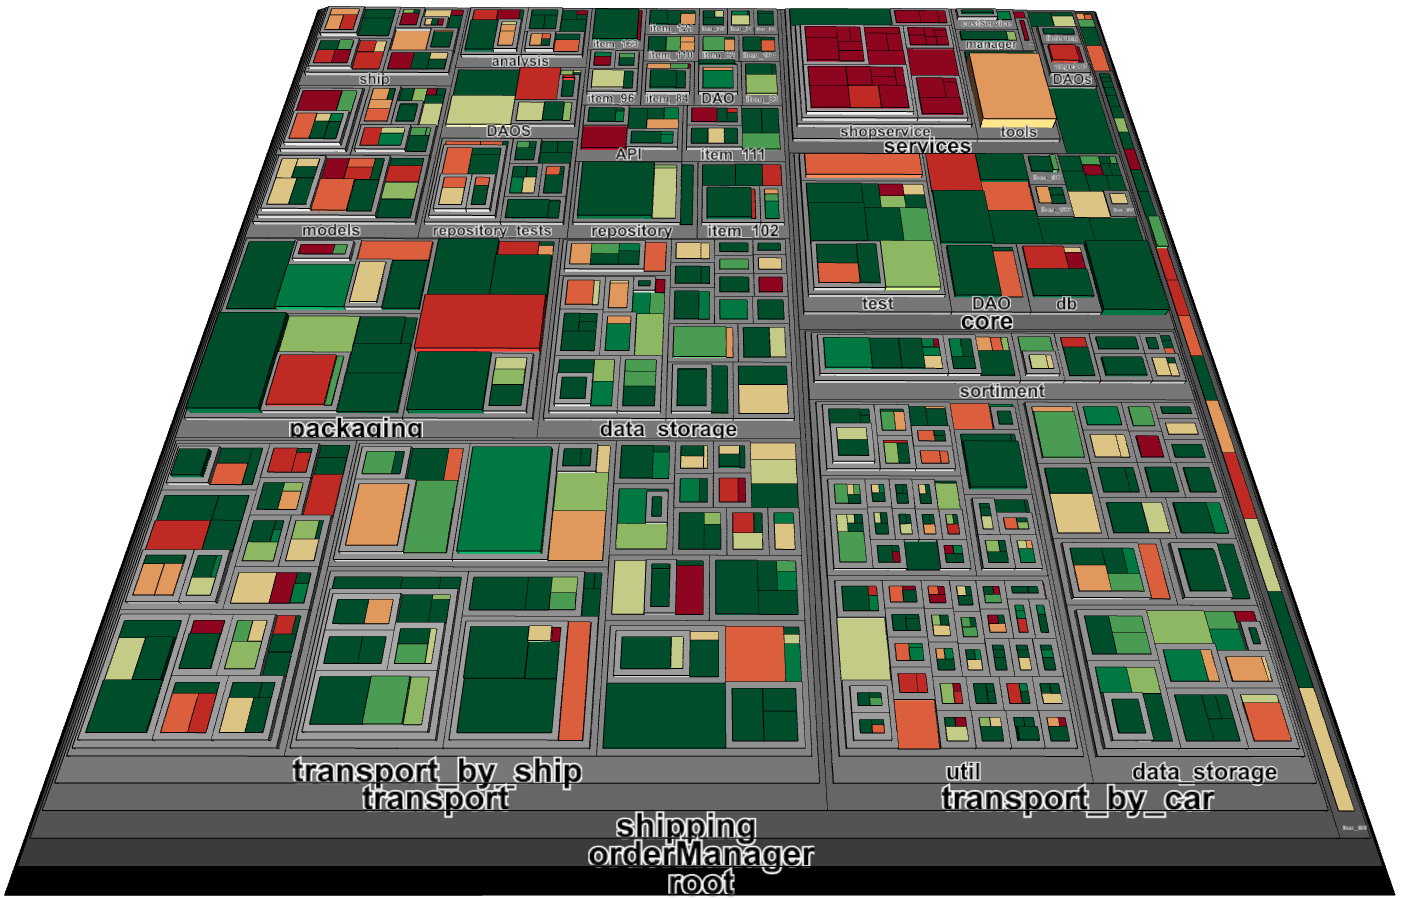
\includegraphics[width=0.8\textwidth]{images/umfrage/treemap/autoren.png}
    \caption[Bild aus Szenario: Autor]{Bild aus Szenario: Stellenweise nur ein Autor, Fläche: Anzahl der Codezeilen, Höhe: Zyklomatische Komplexität, Farbe: Anzahl der Autoren}
\end{figure}

\begin{quote}
    Wie sehr hilft dir die Visualisierung, die Analyse der Experten nachzuvollziehen?
\end{quote}






\subsection*{Szenario: Hohe Komplexität in einzelnen Funktionen}

\begin{quote}
Es ist wichtig, dass Code gut verständlich und wartbar ist. Dazu gehört, dass einzelne Dateien und Funktionen nicht zu komplex sind. Sehr komplexer Code ist schwer zu verstehen, zu testen und zu warten. Komplexität lässt sich durch verschiedene Metriken messen, etwa die zyklomatische Komplexität, die die Anzahl der möglichen Pfade durch eine Funktion angibt. Ab etwa 50 Pfaden wird Code schwer verständlich, ab 100 Pfaden wird er sehr schwer zu navigieren.

Im Code wurden zahlreiche Funktionen identifiziert, die unnötig komplex sind: sehr lange Methoden, stark verschachtelte -Strukturen, fehlende Guard-Clauses und wenige Hilfsfunktionen. Moderne Sprachfeatures wie Switch(-Expressions) oder Pattern Matching werden selten genutzt, sodass Logik häufig unstrukturiert in großen Funktionen zusammengefasst ist. Dies lässt sich klar an der hohen zyklomatischen Komplexität einiger Dateien erkennen. Dateien mit sehr hoher Komplexität sind über die gesamte Codebasis verteilt. Einige wenige Dateien sind extrem komplex (über 200), was die Wartung deutlich erschwert.

Wir empfehlen, speziell die sehr komplexen Dateien zu überarbeiten und zu vereinfachen, die zudem auch noch groß sind.

Legende:
Fläche: Anzahl der Codezeilen (höchster Wert: 2785)
Höhe: Anzahl der Autoren (höchster Wert: 20)
Farbe: Zyklomatische Komplexität (1-524, 10=grün, 200=rot)
\end{quote}

\begin{figure}[H]
    \centering
    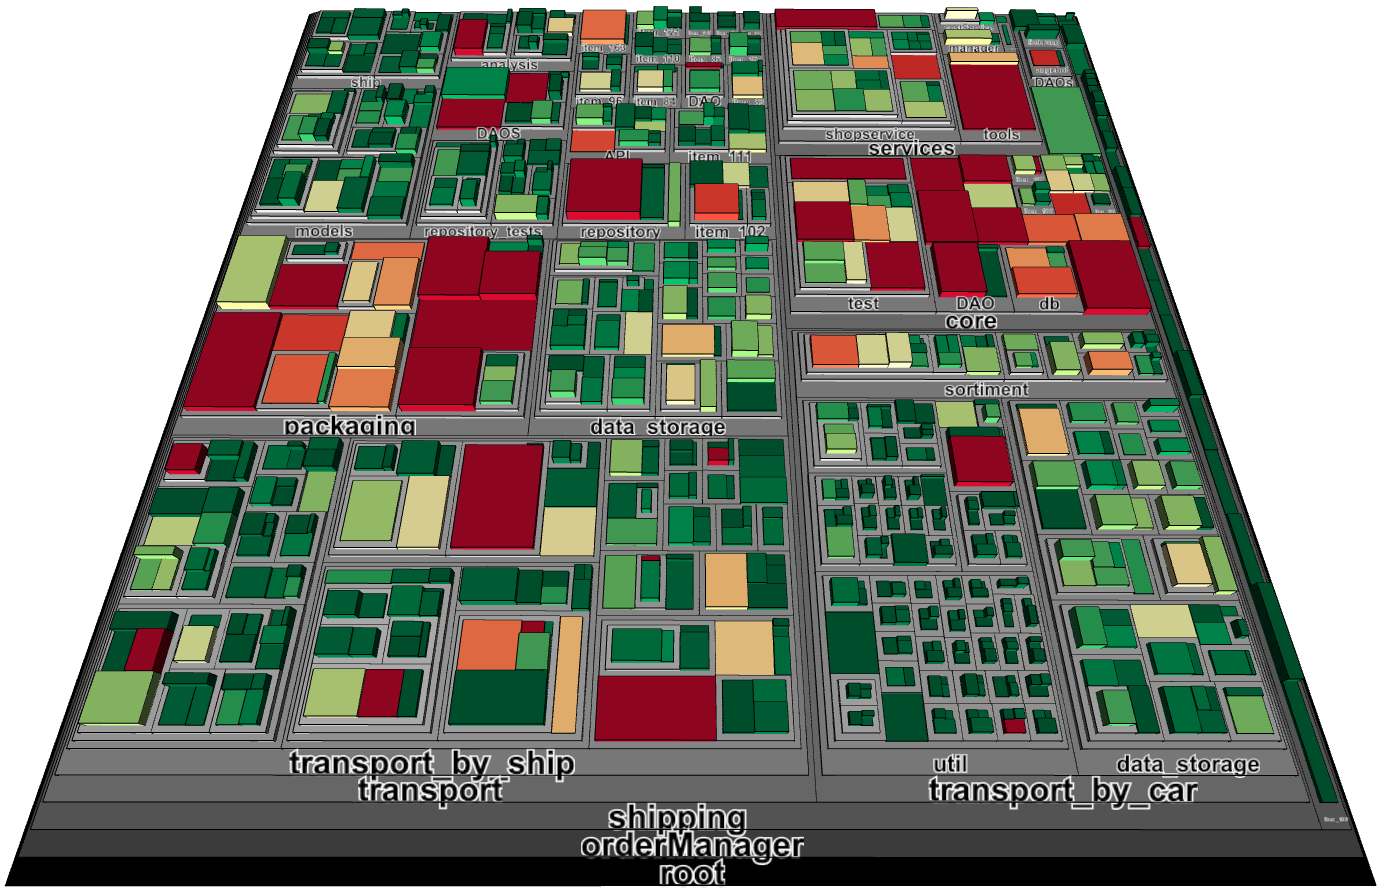
\includegraphics[width=0.8\textwidth]{images/umfrage/treemap/komplex.png}
    \caption[Bild aus Szenario: Hohe Komplexität]{Bild aus Szenario: Hohe Komplexität in einzelnen Funktionen, Fläche: Anzahl der Codezeilen, Höhe: Anzahl der Autoren, Farbe: Zyklomatische Komplexität}
\end{figure}

\begin{quote}
    Wie sehr hilft dir die Visualisierung, die Analyse der Experten nachzuvollziehen?
\end{quote}






\subsection*{Szenario: Komplexe, aber kaum getestete Dateien}

\begin{quote}
Oft reicht es nicht aus, nur eine einzelne Metrik zu betrachten. Manchmal kann zum Beispiel die Komplexität einer Datei akzeptiert werden, wenn man diese dafür gut testet. In diesem Fall ist es wichtig, dass die Tests die komplexe Logik abdecken, damit Fehler früh erkannt werden und die Wartung möglichst wenig Aufwand verursacht. Dies lässt sich durch die Testabdeckung messen, die angibt, wie viel Prozent des Codes durch Tests ausgeführt werden.

Unsere Codeanalyse hat gezeigt, dass einige, der zuvor als zu komplex identifizierten Dateien, nicht vereinfacht werden können, da die zugrunde liegende Logik selbst sehr komplex ist. Einige der komplexen Dateien sind gut getestet, was positiv ist, diese Dateien müssen nicht angepasst werden. Vereinzelt gibt es Ausnahmen, diese Dateien sind jedoch meist klein, sodass der Aufwand zur Behebung von Fehlern gering bleibt. Eine Ausnahme bildet der Ordner "Packaging": Hier liegen viele ungetestete Dateien, von denen einige gleichzeitig groß und sehr komplex sind 

Für den Ordner "Packaging" empfehlen wir daher dringend, die Testabdeckung zu erhöhen.


Legende:
Fläche: Anzahl der Codezeilen (höchster Wert: 2785)
Höhe: Zyklomatische Komplexität (höchster Wert: 524)
Farbe: Testabdeckung in Prozent (0-100, 0 = rot, 100 = grün)
\end{quote}

\begin{figure}[H]
    \centering
    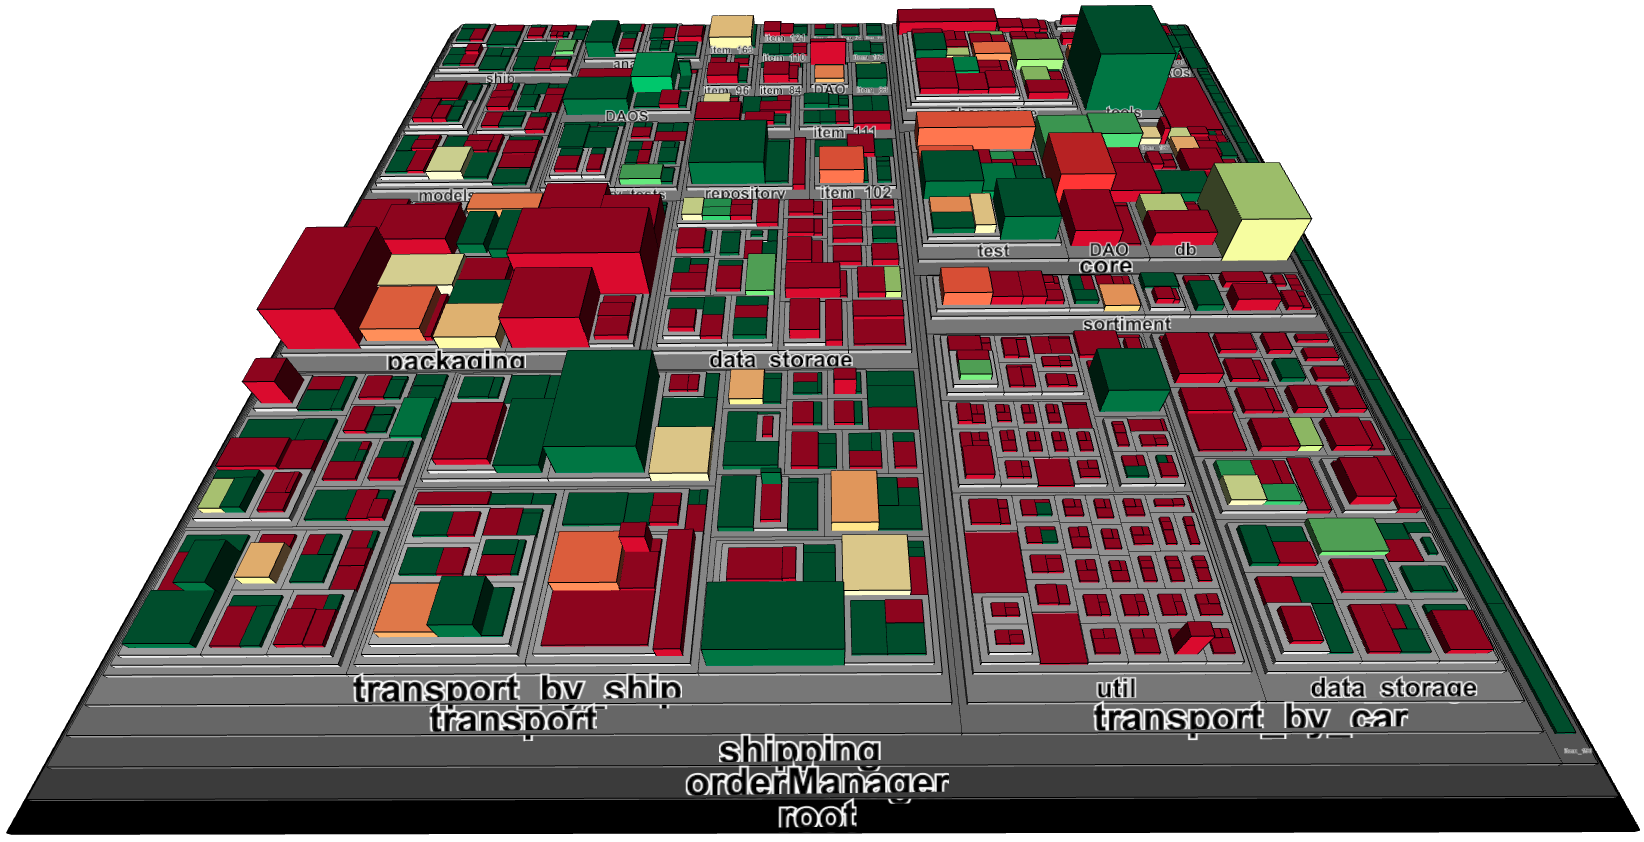
\includegraphics[width=0.8\textwidth]{images/umfrage/treemap/dreierKombi.png}
    \caption[Bild aus Szenario: Komplexe, aber kaum getestete Dateien]{Bild aus Szenario: Komplexe, aber kaum getestete Dateien, Fläche: Anzahl der Codezeilen, Höhe: Zyklomatische Komplexität, Farbe: Testabdeckung in Prozent}
\end{figure}

\begin{quote}
    Wie sehr hilft dir die Visualisierung, die Analyse der Experten nachzuvollziehen?
\end{quote}







\subsection*{Szenario: Kaum Struktur - Ordner enthalten zu viele Dateien}

\begin{quote}
Die Struktur von Softwareprojekten ist entscheidend für die Verständlichkeit und Wartbarkeit. Eine schlechte Struktur erschwert Orientierung, Verantwortlichkeiten und Änderungen. Zu viele Dateien in einem Ordner sind ein Indikator für eine schlechte Struktur, da dies auf fehlende Unterteilung nach Aufgaben oder Features hinweist.


In unserer Codeanalyse ist aufgefallen, dass in mehreren Top-Level-Ordnern sehr viele Dateien liegen, ohne klare Unterteilung nach Aufgaben oder Features. Beim Lesen des Codes fällt auf, dass fachlich nicht zusammengehörige Teile zusammenliegen und große „Allerlei“-Ordner entstanden sind. Viele Ordner enthalten über 13 Dateien, wenige sogar über 30.

Wir empfehlen daher, Ordner entlang von Aufgaben oder Features zu strukturieren und Obergrenzen für die Anzahl von Dateien pro Ordner einzuführen.

Legende:
Fläche: Anzahl der Codezeilen (höchster Wert: 2785)
Höhe: Zyklomatische Komplexität (höchster Wert: 524)
Farbe: Testabdeckung in Prozent (0-100, 0 = rot, 100 = grün)
\end{quote}

\begin{figure}[H]
    \centering
    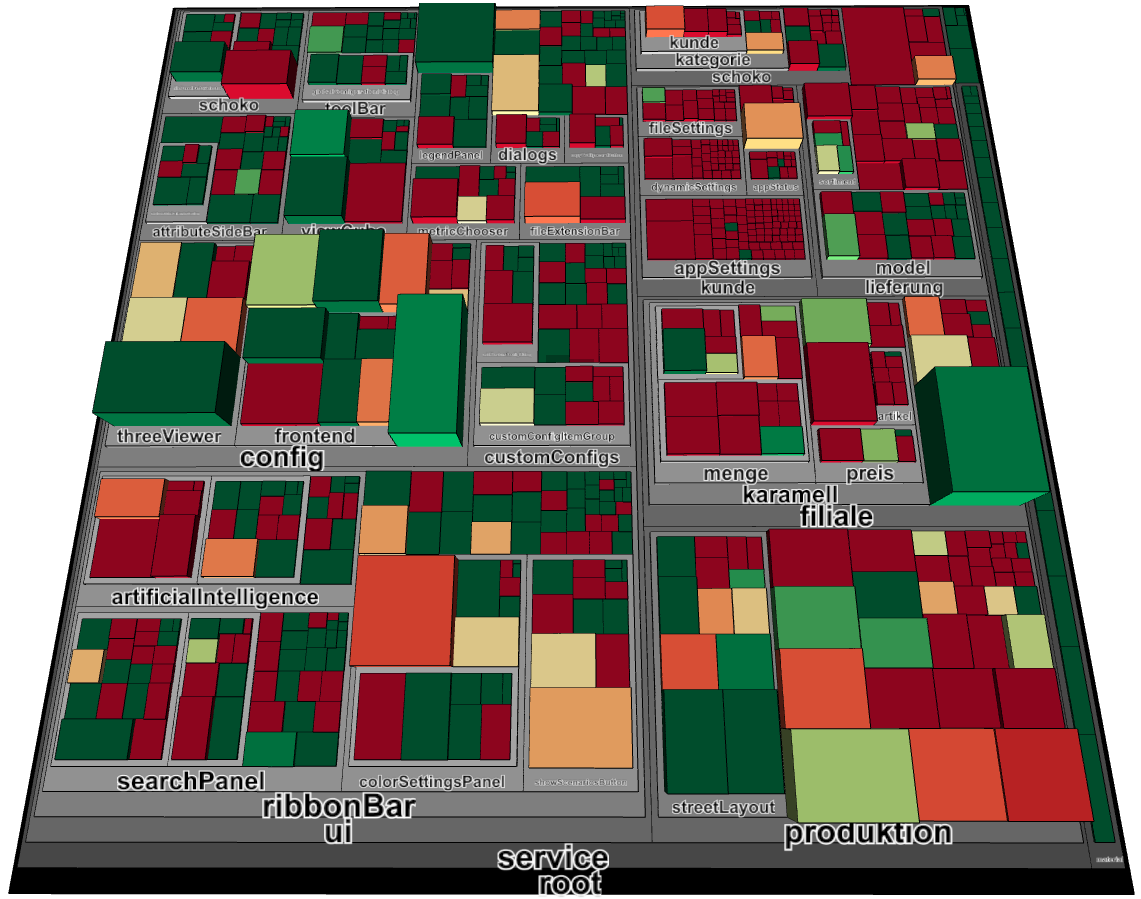
\includegraphics[width=0.8\textwidth]{images/umfrage/treemap/breiteOrdner.png}
    \caption[Bild aus Szenario: Kaum Struktur]{Bild aus Szenario: Kaum Struktur - Ordner enthalten zu viele Dateien, Fläche: Anzahl der Codezeilen, Höhe: Zyklomatische Komplexität, Farbe: Testabdeckung in Prozent}
\end{figure}

\begin{quote}
    Wie sehr hilft dir die Visualisierung, die Analyse der Experten nachzuvollziehen?
\end{quote}





\subsection*{Szenario: Tiefe Verzeichnisstrukturen}

\begin{quote}
Die Struktur von Softwareprojekten ist entscheidend für die Verständlichkeit und Wartbarkeit. Eine schlechte Struktur erschwert Orientierung, Verantwortlichkeiten und Änderungen. Zu tiefe Verzeichnisstrukturen sind ein Indikator für eine schlechte Struktur, da dies auf fehlende klare Ebenen oder zu viele Unterteilungen hinweist. Außerdem erschwert es das Auffinden relevanter Stellen und macht Änderungen langsamer und fehleranfälliger.


Unsere Strukturanalyse hat gezeigt, dass an vielen Stellen die Verzeichnisstruktur 7-10 Ebenen tief ist. Beim Navigieren durch den Code fallen lange Pfade, Ordner mit nur einer Datei und stark verschachtelte Unterordner auf. 

Wir empfehlen daher, manuell die Struktur abzuflachen und lange Pfadketten zu vermeiden. Zudem empfehlen wir Obergrenzen für die Tiefe der Verzeichnisstruktur einzuführen und sinnvolle, breit gefasste Ebenen mit klaren Namen zu nutzen. 

Legende:
Fläche: Anzahl der Codezeilen (höchster Wert: 2785)
Höhe: Zyklomatische Komplexität (höchster Wert: 524)
Farbe: Testabdeckung in Prozent (0-100, 0 = rot, 100 = grün)
\end{quote}

\begin{figure}[H]
    \centering
    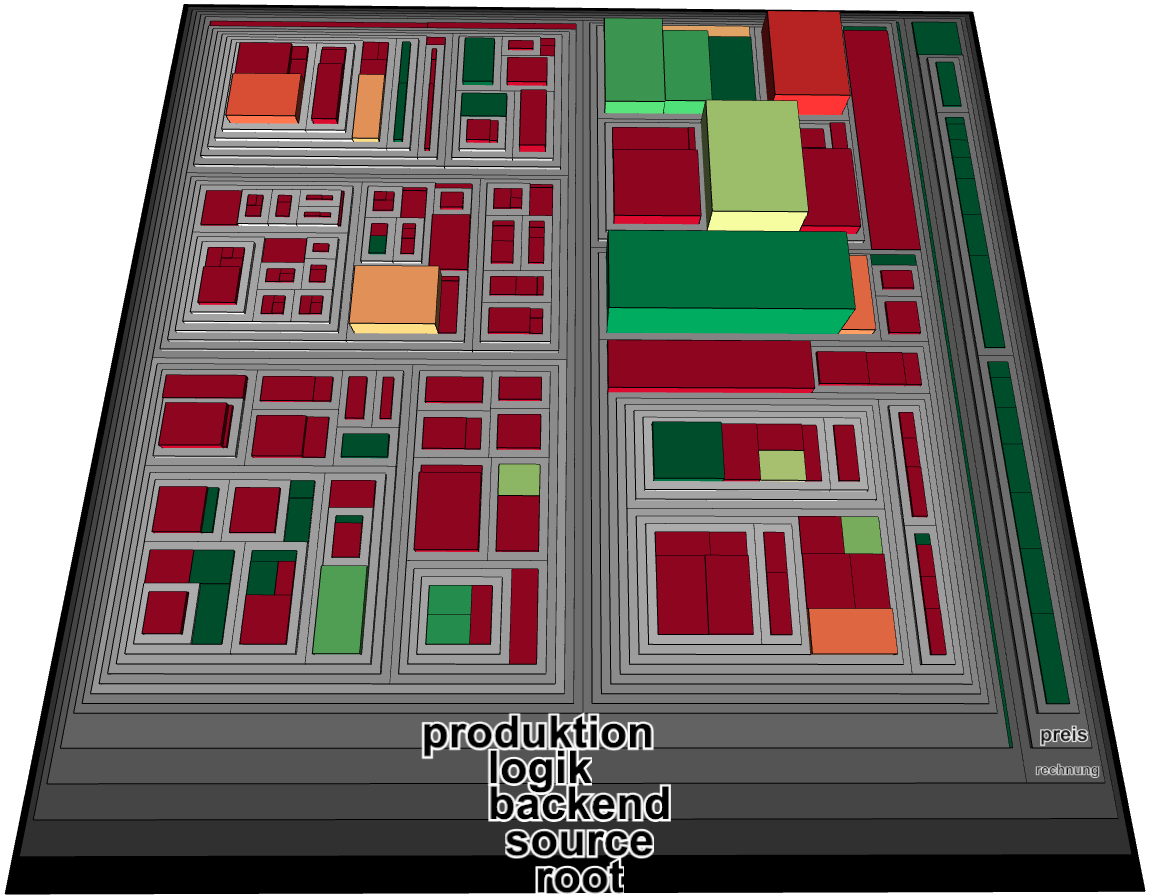
\includegraphics[width=0.8\textwidth]{images/umfrage/treemap/tiefeOrdner.png}
    \caption[Bild aus Szenario: Tiefe Verzeichnisstrukturen]{Bild aus Szenario: Tiefe Verzeichnisstrukturen, Fläche: Anzahl der Codezeilen, Höhe: Zyklomatische Komplexität, Farbe: Testabdeckung in Prozent}
\end{figure}

\begin{quote}
    Wie sehr hilft dir die Visualisierung, die Analyse der Experten nachzuvollziehen?
\end{quote}






\subsection*{Szenario: Schlechte Architektur und uneinheitliche Benennungen}

\begin{quote}
Das Architektur Prinzip, nach dem die analysierte Software entwickelt wurde ist das Domain Driven Design Prinzip. Es besagt, dass sich Software nach fachlichen Prinzipien richtet und nicht nach technischen Prinzipien. Fachliche Prinzipien sind zum Beispiel die fachlichen Aufgaben wie Transport, Lagerung oder Bestellung. Diese Struktur sollte sich in der Ordnerstruktur sinnvoll widerspiegeln. Außerdem ist es wichtig einheitliche Bennennungen über die ganze Codebasis zu verwenden, damit klar ist, wie etwas zu finden ist. Wenn dies nicht der Fall ist, spricht das für eine schlechte Architektur, was die Wart- und Erweiterbarkeit erschwert.

Unsere Architekturanalyse hat gezeigt, dass fachliche Grenzen entweder nicht sauber eingehalten werden oder gar nicht erst existieren. Beim Lesen des Codes fallen fachfremde Abhängigkeiten und das „Durchreichen“ von Daten auf, die dort nichts zu suchen haben. Zum Beispiel finden sich in der Transport-Logik ("transport") Abhängigkeiten zur Verpackungs-Logik ("packaging"). Zudem liegt die Transport-Logik per Auto ("transport_by_car") nicht unter dem fachlichen Kontext Transport ("transport") sondern auf der gleichen Ebene wie dieser. 
Auffallend (aber einfach zu beheben) sind auch uneinheitliche Benennungen, wie zum Beispiel Data Access Objects. Teilweise werden diese DAO, DAOs oder DAOS genannt. Zudem sind die Namensgebungen uneinheitlich: Teilweise werden Wörter mit Unterstrich getrennt, teilweise mit Groß- und Kleinschreibung.

Wir empfehlen daher, Richtlinien für die Benennung einzuführen und diese konsequent anzuwenden. Zudem empfehlen wir, die gesamte Architektur zu überarbeiten, indem fachliche Grenzen (Bounded Contexts) definiert und mit Architekturtests versehen werden. Code sollte entlang dieser fachlichen Grenzen neu strukturiert werden und Querverbindungen sollten nur über klar definierte Schnittstellen oder Adapter erfolgen.

Legende:
Fläche: Anzahl der Codezeilen (höchster Wert: 2785)
Höhe: Zyklomatische Komplexität (höchster Wert: 524)
Farbe: Testabdeckung in Prozent (0-100, 0 = rot, 100 = grün)
\end{quote}

\begin{figure}[H]
    \centering
    \includegraphics[width=0.8\textwidth]{images/umfrage}
    \caption[Bild aus Szenario: Schlechte Architektur und uneinheitliche Benennungen]{Bild aus Szenario: Schlechte Architektur und uneinheitliche Benennungen, Fläche: Anzahl der Codezeilen, Höhe: Zyklomatische Komplexität, Farbe: Testabdeckung in Prozent}
\end{figure}

\begin{quote}
    Wie sehr hilft dir die Visualisierung, die Analyse der Experten nachzuvollziehen?
\end{quote}







\subsection*{Szenario: Duplikation}

\begin{quote}
In der Softwareentwicklung gibt es das Prinzip „Don't Repeat Yourself“ (DRY), welches besagt, dass sich Code nicht duplizieren sollte. Duplizierter Code erschwert die Wartung, da Fehler an mehreren Stellen behoben werden müssen und Änderungen inkonsistent umgesetzt werden können. Zudem vergrößert sich die Codebasis unnötig, was die Verständlichkeit erschwert.

Unsere Analyse zeigt, dass die beiden "data_storage" Ordner nahezu den gleichen Inhalt besitzen: gleiche Struktur, ähnliche Datei- und Klassennamen sowie kopierter Code mit kleinen Abweichungen. Unsere Duplikationsanalyse zeigt eine hohe Ähnlichkeit (>80 Prozent gleiche Tokens).

Wir empfehlen daher, die Duplikationen zu entfernen und den gemeinsamen Code in ein wiederverwendbares Modul zu extrahieren. Nur die wirklich spezifischen Teile sollten getrennt bleiben. Zudem empfehlen wir, Duplikationsprüfungen in die CI aufzunehmen, um künftige Duplikationen frühzeitig zu erkennen.


Legende:
Fläche: Anzahl der Codezeilen (höchster Wert: 2785)
Höhe: Zyklomatische Komplexität (höchster Wert: 524)
Farbe: Testabdeckung in Prozent (0-100, 0 = rot, 100 = grün)
\end{quote}

\begin{figure}[H]
    \centering
    \includegraphics[width=0.8\textwidth]{images/umfrage}
    \caption[Bild aus Szenario Duplikation]{Bild aus Szenario Duplikation, Fläche: Anzahl der Codezeilen, Höhe: Zyklomatische Komplexität, Farbe: Testabdeckung in Prozent}
\end{figure}

\begin{quote}
    Wie sehr hilft dir die Visualisierung, die Analyse der Experten nachzuvollziehen?
\end{quote}